\documentclass[11pt,a4paper]{article}
\usepackage[T1]{fontenc}
\usepackage[utf8]{inputenc}
\usepackage{lmodern,microtype}
\usepackage[margin=25mm]{geometry}
\usepackage{amsmath,amssymb,booktabs,tabularx,longtable,array,graphicx}
\usepackage[dvipsnames]{xcolor}
\definecolor{burgundy}{HTML}{741E35}
\usepackage{titlesec}
\titleformat{\section}{\large\bfseries\color{burgundy}}{\thesection}{.7em}{}
\titleformat{\subsection}{\normalsize\bfseries\color{burgundy}}{\thesubsection}{.7em}{}
\usepackage[authoryear,round]{natbib}
\usepackage[colorlinks=true,linkcolor=burgundy,citecolor=burgundy,urlcolor=burgundy,breaklinks=true]{hyperref}
\usepackage{fancyhdr}
\pagestyle{fancy}\fancyhf{}\fancyhead[L]{\small What does identity-linked information buy?}\fancyhead[R]{\small Draft}\fancyfoot[C]{\thepage}
\setlength{\headheight}{15pt}
\usepackage{float}
\hypersetup{pdftitle={What Does Identity-Linked Information Buy?},pdfauthor={Murad Farzulla and Andrew Maksakov},pdfsubject={Synthetic payment monitoring: September 2026 draft},pdfkeywords={CBDC, payment monitoring, synthetic data, data minimization}}
\setlength{\parskip}{4pt}\setlength{\parindent}{1em}
\newcommand{\AP}{\operatorname{AP}}
\newcommand{\Miss}{\operatorname{MissedPer10k}}
\title{\color{burgundy}\bfseries What Does Identity-Linked Information Buy?\\[5pt]\large Detector Flexibility and Review Budgets in Synthetic Payment Monitoring}
\author{Murad Farzulla\thanks{Correspondence: \href{mailto:murad@dissensus.ai}{murad@dissensus.ai}. ORCID: \href{https://orcid.org/0009-0002-7164-8704}{0009-0002-7164-8704}.} \quad Andrew Maksakov\\[3pt]\small Dissensus, London, United Kingdom}
\date{12 September 2026\\\small Draft for scientific review; DAI-2511 revision candidate}
\begin{document}
\maketitle
\begin{abstract}
The detection value of customer information is often discussed without separating pseudonymous wallet linkage, customer attributes, and watchlist membership. We estimate these increments in a synthetic payment-monitoring experiment and distinguish ranking performance from the number of illicit entities missed at a fixed review budget. Across 52 independently generated training and test population pairs, adding customer attributes and a watchlist to oracle linkage reduces missed illicit entities per 10,000 by 7.90 (90\% interval 7.13--8.68) for gradient boosting and 31.35 (29.93--32.76) for logistic regression, at 500 reviews per 10,000. Customer attributes alone account for 2.40 and 14.85 of these reductions, respectively. A separate replicated four-model experiment finds that much of the smaller auxiliary-information increment is already present with additive nonlinear models; additional interactions do not produce a monotonic reduction. All four models benefit when auxiliary signals are strengthened. The originally proposed budget of 50 reviews was saturated in every pilot replicate. No policy tolerance was fixed, so no non-inferiority claim is made; a recovered gatekeeping defect also prevents calling the model contrast confirmatory. These results measure conditional detection costs in specified synthetic regimes. They neither establish that identity collection is dispensable nor validate a privacy-preserving deployment. We develop the institutional implications of separating wallet linkage from identity resolution, with a centralized baseline and an optional threshold-authorized resolution design.
\end{abstract}
\noindent\textbf{Keywords:} payment monitoring; synthetic data; anti-money laundering; central bank digital currency; data minimization; model comparison.

\section{Introduction}
An institution can know that several wallets belong together without routinely attaching a civil identity to the resulting transaction history. Conversely, knowing a customer's name need not reveal behavioral patterns distributed across accounts. These are different information capabilities. A useful empirical question is how much detection performance each capability adds, conditional on the detector, the population, and the number of alerts investigators can review.

This question matters for central bank digital currency (CBDC) design, but is broader than CBDCs. It concerns the organization of information in any payment-monitoring system. Projects Aurora and Hertha already demonstrate that collaborative and network-level analytics can contribute to detection in synthetic payment data \citep{Aurora,Hertha}. Cryptographic payment systems already combine privacy with selected regulatory functions \citep{Platypus,PEReDi,Pools}. Our contribution is a measurement exercise within that established problem: hold the generated population and model family fixed, add defined information blocks, and estimate the resulting changes in detection and missed cases. We do not claim to have discovered privacy-compatible compliance or invented a new cryptographic primitive.

The central result is a conditional pattern. In our default generator, nonlinear detectors use linked behavioral aggregates more effectively than logistic regression, and consequently gain less from additional customer attributes and watchlist access. Less is not zero. The replicated estimates are positive for both models, and the information gains rise when the generator gives auxiliary attributes stronger signal. The four-model comparison further narrows the interpretation: additive nonlinear models already exhibit the smaller increment, while unconstrained boosting does not uniformly improve on the additive model. A claim about an invariant value of identity, or a monotonic law of model capacity, would exceed these results.

We also contribute an operational diagnostic. A review budget can force apparently favorable comparisons to zero when all models select only positive cases. In the excluded pilot, 50 reviews per 10,000 produced exactly zero differences in every replicate. Reporting that endpoint as proof of non-inferiority would have reproduced the structure of the earlier measurement error this revision corrects. We therefore report an informative budget, disclose its pilot-dependent selection, and leave the acceptability of the measured detection loss unevaluated because no defensible tolerance was specified.

The article brings together two complementary experiments. The first evaluates fixed models on independently generated training and test populations. The second maps information increments across four model families and several generator regimes using nested cross-validation. They answer related questions but use different training and evaluation procedures; their numerical outputs are not interchangeable. Both concern synthetic entities with an oracle wallet map. The accompanying institutional design is an implication to examine, not a system tested by either experiment.

\section{Background and scope}
\subsection{Detection and regulated privacy}
Project Aurora studies collaborative analysis, privacy-enhancing technologies, and machine learning for detecting synthetic laundering patterns across institutional boundaries \citep{Aurora}. Project Hertha compares payment-system analytics with the information available to banks and payment service providers, and studies their combination \citep{Hertha}. These projects motivate attention to information access, but their monitoring scenarios bundle several differences. Our controlled feature tiers instead distinguish entity linkage from customer attributes and a watchlist under one generator. This distinction describes our experimental design; it is not a systematic claim that no previous study has performed any comparable ablation.

Platypus builds privacy-preserving regulation into a CBDC design using an e-cash approach and a centralized trust model \citep{Platypus}. PEReDi formalizes a distributed CBDC with regulated tracing and auditing \citep{PEReDi}. Privacy Pools permits proofs about association sets without exposing an entire transaction history \citep{Pools}. These constructions have different privacy, functionality, and trust assumptions. Their existence precludes treating the mere combination of privacy and compliance as our novelty. Our proposed role separation borrows established ideas but does not inherit a security proof merely by citing them.

The empirical outcome is the recovery of generator-assigned illicit labels. It does not measure successful investigation, adjudicated crime, prevented harm, user welfare, or the lawfulness of collecting a field. A previous suspicious-activity-report count is an experimentally assigned predictor here; it is not assumed to be an unbiased real-world measure of criminality. Names and government identifiers never enter the models. Accordingly, the term \emph{identity-linked information} means the specified customer-attribute block and, where stated, the watchlist. It does not mean that naming a person itself produces the measured gain.

\subsection{Correction and evidential status}
This paper replaces the empirical interpretation of earlier versions of DAI-2511. The original generator separated legitimate and illicit entities by wallet counts and could produce perfect single-feature classification. Its detection percentages and claim of no watchlist value are withdrawn. A corrected single-seed analysis was subsequently released, but it was not an adequate basis for statements about all detectors or operating points. The present draft reports replicated results and distinguishes customer attributes from the combined attribute-plus-watchlist block throughout.

The August protocols were specified in advance of their respective frozen runs, but no completed public preregistration is evidenced by the repository. We use \emph{pre-specified}, not \emph{preregistered}. A September audit also found that the independent-population driver bypassed its own hierarchical testing rule when the non-inferiority tolerance was absent. The raw outcomes and intervals remain usable; the corresponding confirmatory claim does not. Section~\ref{sec:inference} explains the correction. Other departures from the ladder protocol are disclosed in Section~\ref{sec:deviations}, so a planned analysis is not mistaken for an executed one.

\section{Materials and methods}
\subsection{Synthetic populations}
The generator creates legitimate and illicit entities, wallets, and time-stamped positive-value transactions over 120 simulated days. In the default population, each entity independently receives an illicit label with probability 0.05. Both classes draw wallet counts from the same distribution, $1+\operatorname{Binomial}(5,0.30)$. This removes the original definitional wallet-count separator. The population also includes a shared pool of 3,000 external wallet identifiers.

Legitimate activity mixes saver, spender, and business profiles. Income, spending, self-transfers, large purchases, and payroll-sized outflows introduce overlap with laundering signatures. Illicit entities receive cover activity plus placement, layering, and integration cycles. At the default obfuscation setting of 0.6, placement smurfing occurs with probability 0.60 when the amount exceeds the generator's placement condition; integration-side structuring follows a separate probability, 0.46 at that setting. The simulated reporting threshold is 10,000 units of account. It is a generator parameter, not a statement of a jurisdiction's reporting law.

Customer attributes are sampled from overlapping class-conditional distributions. They comprise KYC tier, account age, previous suspicious-activity-report count, and jurisdiction risk. Watchlist inclusion has default probabilities 0.40 for illicit and 0.02 for legitimate entities. These signal strengths are chosen by the experimenters; they are not estimated from confidential banking data. The generator therefore allows a controlled question about conditional information value without identifying its magnitude in a real payment population. Complete parameters and source hashes accompany the results.

\subsection{Information tiers and comparison unit}
Table~\ref{tab:tiers} defines the information sets. T2, T3, and T4 are nested. T1 is a separate wallet-level benchmark, with a different representation and evaluation procedure; it is not a feature subset of T2.
\begin{table}[htbp]\centering\small
\caption{Information available to the detector. No tier contains a civil name or government identifier.}\label{tab:tiers}
\begin{tabularx}{\linewidth}{lX}\toprule
Tier & Operational definition \\\midrule
T1 & Sixteen per-wallet transaction features. Wallets are scored separately; evaluation takes the maximum wallet score within each true entity. This aggregation uses the oracle entity map only for evaluation. \\
T2 & Nineteen entity-level behavioral features, including linked-wallet timing and flow aggregates, internal transfers, external counterparties, and cross-wallet pass-through. The true wallet-to-entity map is supplied. \\
T3 & T2 plus KYC tier, account age, previous suspicious-activity-report count, and jurisdiction risk. \\
T4 & T3 plus a binary watchlist indicator. \\\bottomrule
\end{tabularx}
\end{table}

T2 measures an idealized linked representation, denoted T2-oracle. No entity-resolution algorithm estimates that map. A stable entity cluster already supports longitudinal surveillance even without a civil name. Moreover, T1's oracle aggregation makes it unsuitable as a direct estimate of the cost of operating an unlinked alert queue. We retain its scores in the data for continuity but base the substantive incremental claims on T2--T4. The comparison does not assign a numerical privacy score to any tier.

For a higher-is-better ranking metric $M$, define
\begin{align}
\Delta_I(M)&=M(\mathrm{T3})-M(\mathrm{T2}),\\
\Delta_W(M)&=M(\mathrm{T4})-M(\mathrm{T3}),\\
\Delta_F(M)&=M(\mathrm{T4})-M(\mathrm{T2})=\Delta_I(M)+\Delta_W(M).
\end{align}
The subscript $I$ denotes the four customer attributes, $W$ the watchlist, and $F$ their combined increment above linkage. Each tier is fitted separately. These are fitted-model performance differences, not conditional mutual information or a causal effect of a person's identity.

\subsection{Operational endpoint and independent populations}
Each of 52 replicates generates 8,000 training entities and an independent population of 10,000 test entities. Training and test random streams are disjoint, with a fixed offset of 10,000,003. We fit logistic regression with standardization and balanced class weights, and histogram gradient boosting with balanced class weights, to T2, T3, and T4 separately. These fixed-model experiments use no test-dependent tuning. The repository pins NumPy 2.3.5, SciPy 1.16.3, pandas 2.3.3, and scikit-learn 1.8.0.

The budget selects the $k$ highest-scoring entities, breaking ties by numeric entity identifier. With test labels $Y_e$ and selected set $A_k$, the operational outcome is
\begin{equation}
\Miss(m,t;k)=\frac{10,000}{n}\left[\sum_{e=1}^{n}Y_e-\sum_{e\in A_k(m,t)}Y_e\right].
\end{equation}
Our primary contrast is $D_{F,m}=\Miss(m,\mathrm{T2};k)-\Miss(m,\mathrm{T4};k)$. Positive values mean additional information reduces missed illicit entities. The analogous T2--T3 and T3--T4 differences report the attribute and watchlist components. All comparisons are paired within the same test population. At $n=10,000$, one unit is one additional missed illicit entity, not a percentage point of recall.

An excluded 20-replicate pilot examined budgets and estimated between-replicate variability. Its seeds, 900001--900020, are permanently excluded from the 52-replicate analysis. The proposed budget of 50 per 10,000 was saturated: both models' compared tiers selected 50 positive cases in every pilot replicate, so their difference was exactly zero. The final budget, 500 per 10,000, was chosen after this pilot and before the independent-population run. Precision targets of 1.0 for the boosted full-access contrast and 2.5 for the between-model contrast were also fixed post-pilot. These are interval half-width targets used for sample sizing, not tolerances for an acceptable loss of detection. The final lock deliberately leaves that policy tolerance unset.

\subsection{Inference and the recovered gatekeeping error}\label{sec:inference}
For each contrast we summarize the independent replicate values $D_1,\ldots,D_R$ by their mean, standard deviation, and the pointwise interval
\begin{equation}
\overline D\ \pm\ t_{0.95,R-1}\frac{s_D}{\sqrt{R}}.
\end{equation}
This is a two-sided 90\% Student-$t$ interval for the replicate mean. It does not describe the range of individual worlds and does not provide simultaneous coverage for all cells, tiers, and model comparisons. The accompanying data also report medians and interquartile ranges as between-world variation. Small-$R$ sensitivity cells warrant correspondingly limited interpretation.

The original testing plan placed a non-inferiority hypothesis H1 before a model-moderation hypothesis H2. H2 could be confirmatory only if H1 established non-inferiority against a fixed tolerance. Because the lock left that tolerance absent, H1 returned \texttt{ESTIMATE\_ONLY}. The driver nevertheless passed \texttt{NON\_INFERIOR} to the H2 gate. This was an implementation error: an absent tolerance cannot establish non-inferiority. We corrected the driver to pass the actual H1 status, retained the original raw records, and report the model contrast descriptively. Neither H1 nor H2 is rescued by choosing a tolerance after seeing these results. The correction changes the evidential status, not the numerical contrast.

Failed replicates are counted and logged without replacing their seeds. The final 52-replicate run has no failures. Before that run, an invalid out-of-range random-state base caused a failed attempt; the archived lock records its correction before any valid outcomes existed. This history does not supply missing preregistration or justify bypassing the gate.

\subsection{Four-model and generator-regime experiment}
The second experiment compares logistic regression (linear), histogram boosting constrained to additive feature effects, a random forest, and unconstrained histogram boosting. Every model family has four candidate configurations. Three-fold stratified inner cross-validation selects by average precision on T4 within each outer training fold; that selected configuration is reused across tiers in that fold. All entities are disjoint across the five outer folds, and all wallets inherit their entity's fold. See Appendix~\ref{app:models} for the grids.

Average precision (AP) is computed on concatenated out-of-fold scores. Operational recall, precision, and missed cases are also calculated at a 5\% entity review budget. This procedure evaluates a cross-validated ranking within a generated population. Different fold models may produce differently scaled probabilities, and global out-of-fold ranking can therefore depend on calibration across folds. The independent-population experiment avoids that particular issue and carries the principal operational result. Shared tuning on T4 controls the tuning budget but is not necessarily optimal for T2; it can favor configurations selected for richer information. Hyperparameter configurations and outcomes are retained for inspection.

The default cell has 20 independently generated worlds. A surface varies behavioral obfuscation over 0.9, 0.6, and 0.3 (low, medium, and high behavioral recoverability) and auxiliary signal over low, medium, and high. Low signal makes the specified attribute and watchlist distributions equal across classes; medium is the default; high strengthens the auxiliary block. Every nondefault surface cell has 10 replicates. All surface cells were actually run at 5\% prevalence. Default-regime cells at 1\% and 3\% each add 10 replicates. A separate positive-control world combines strong auxiliary information with weaker behavioral signals and has two replicates. These 122 world-replicate units each contain all four models; they are not 122 independent replications of each surface cell.

Changing obfuscation changes cover activity as well as laundering signatures. Changes to class-conditional attribute sampling can also alter the downstream random stream. Consequently, the surface is a comparison of generated regimes, not a paired causal intervention isolating one pure mechanism. We estimate model contrasts using paired values within a world and do not infer an isolated causal effect of ``capacity'' from differences between model families.

\subsection{Diagnostics and departures from the ladder plan}\label{sec:deviations}
Before fitting an eligible original world, the audit checks the AUC of each individual feature (allowing sign reversal) and rejects a single-feature AUC above 0.95; a second check rejects class-disjoint entity-feature marginals. The independent-population experiment applies this gate to training data only. These checks catch the original wallet-count artifact but do not exclude multivariate separability, realistic-looking label leakage, or a generator poorly representative of practice. There were no gate exclusions among the 122 frozen ladder units.

The written ladder protocol named 3\% prevalence for the surface, while the driver and all 80 nondefault surface records use 5\%. We report the executed 5\% experiment and disclose this unamended deviation. The proposed eight-cell factorial ablation and default within-replicate bootstrap were not implemented and contribute no evidence here. We use between-world intervals only. Earlier notes describing the entire expansion as completed overstated what ran.

The ladder's promised per-world permutation controls were also absent. We added these retrospectively in September: two fresh label-permuted worlds for each of the nine 5\% surface cells and the two additional prevalence cells, with the same four-model nested procedure. Labels are permuted at entity level after generating features and before splitting, tuning, fitting, and evaluation. These 22 diagnostic runs are reported as retrospective controls, not part of the original frozen result. We additionally reproduced all 52 independent-population records and one complete original default ladder unit from their original seeds. Reproduction checks compare raw outcomes and selected configurations, not merely rounded manuscript values.

\section{Results}
\subsection{Additional information reduces missed cases}
Table~\ref{tab:independent} reports the component and total reductions in missed illicit entities. For gradient boosting, withholding the combined customer-attribute and watchlist block costs 7.90 additional misses per 10,000 test entities. The corresponding logistic-regression cost is 31.35. Both intervals lie above zero. The descriptive difference between these gains is 23.44 [21.83, 25.05] misses per 10,000. It is a between-model difference in information gains, not a difference in the models' total performance.
\begin{table}[htbp]\centering\small
\caption{Independent-population estimates: reduction in missed illicit entities per 10,000 at 500 reviews. Means and pointwise 90\% intervals over 52 paired replicates. No non-inferiority verdict is assigned.}\label{tab:independent}
\begin{tabular}{lccc}\toprule Model & Attributes (T2--T3) & Watchlist (T3--T4) & Full block (T2--T4) \\\midrule
Logistic & 14.85 [13.64, 16.06] & 16.50 [15.42, 17.58] & 31.35 [29.93, 32.76] \\
Boosted & 2.40 [1.88, 2.93] & 5.50 [4.71, 6.29] & 7.90 [7.13, 8.68] \\
\bottomrule
\end{tabular}
\end{table}

Customer attributes alone reduce missed cases by 2.40 [1.88, 2.93] for boosting and 14.85 [13.64, 16.06] for logistic regression. The watchlist contributes 5.50 [4.71, 6.29] and 16.50 [15.42, 17.58], respectively. Combining these channels and calling the result the value of identity alone would obscure both effects. Table~\ref{tab:levels} gives the absolute missed-case levels so that a smaller increment is not mistaken for the absence of remaining detection failures.
\begin{table}[htbp]\centering\small
\caption{Absolute missed illicit entities per 10,000, with pointwise 90\% intervals, in the independent-population experiment.}\label{tab:levels}
\begin{tabular}{lccc}\toprule Model & T2 linkage & T3 + attributes & T4 + watchlist \\\midrule
Logistic & 111.44 [108.41, 114.47] & 96.60 [93.81, 99.38] & 80.10 [77.39, 82.80] \\
Boosted & 43.29 [41.27, 45.31] & 40.88 [38.81, 42.96] & 35.38 [33.27, 37.50] \\
\bottomrule
\end{tabular}
\end{table}
\begin{figure}[htbp]\centering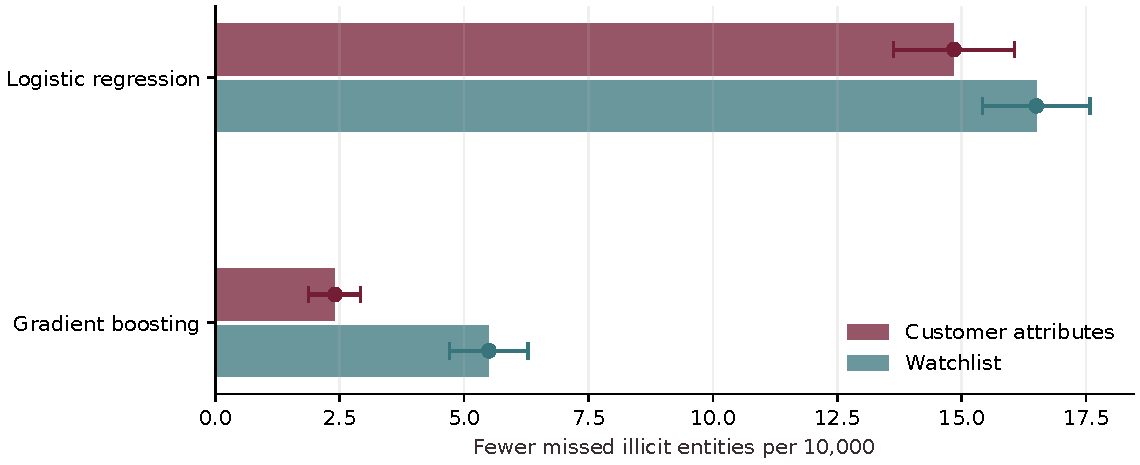
\includegraphics[width=.94\linewidth]{figures/independent.pdf}\caption{Customer-attribute and watchlist increments on the operational endpoint. Bars are paired mean reductions in missed cases; points and whiskers show means and pointwise 90\% intervals.}\label{fig:independent}\end{figure}

\subsection{Much of the change appears with additive nonlinear models}
At default settings, the full-access AP increment is 0.0570 for logistic regression, 0.0128 for additive boosting, 0.0125 for the forest, and 0.0160 for unconstrained boosting (Table~\ref{tab:ladder}). The nonlinear models already rank linked behavior highly: mean T2 AP ranges from approximately 0.951 to 0.959, compared with 0.858 for logistic regression. Small additional gains therefore coexist with limited remaining AP headroom. They are not evidence that auxiliary variables contain no useful information.
\begin{table}[htbp]\centering\small
\caption{Default four-model experiment: AP increments, 20 independent worlds per model; pointwise 90\% intervals. AP is on its native 0--1 scale.}\label{tab:ladder}
\begin{tabular}{lccc}\toprule Model & $\Delta_I$ & $\Delta_W$ & $\Delta_F$ \\\midrule
Linear & 0.0272 [0.0243, 0.0301] & 0.0298 [0.0272, 0.0325] & 0.0570 [0.0528, 0.0612] \\
Additive & 0.0037 [0.0027, 0.0048] & 0.0090 [0.0075, 0.0105] & 0.0128 [0.0110, 0.0145] \\
Forest & 0.0043 [0.0034, 0.0051] & 0.0082 [0.0065, 0.0099] & 0.0125 [0.0104, 0.0145] \\
Boosted & 0.0070 [0.0056, 0.0085] & 0.0089 [0.0068, 0.0111] & 0.0160 [0.0135, 0.0184] \\
\bottomrule
\end{tabular}
\end{table}

The difference between the linear and additive full-access increments is much larger than the difference between the additive and unconstrained boosting increments. In fact, unconstrained boosting has a slightly larger mean auxiliary-information increment than additive boosting. Thus, the data support the descriptive observation that flexible marginal responses already capture much of the available behavioral signal. They do not isolate a unique causal mechanism or establish a monotonic relationship between model complexity and information substitution. The algorithms, regularization, and optimization procedures differ as well as their representational flexibility.

The operational ladder results retain the same broad separation between logistic regression and the nonlinear models (Table~\ref{tab:ladderops}). They also show why reporting only AP is inadequate: the quantity of interest for an investigator may be additional missed cases at the actual alert budget, even when an AP change looks numerically small.
\begin{table}[htbp]\centering\small
\caption{Cross-validated default-world operational results at a 5\% alert budget. These are distinct from the independently generated test-population experiment.}\label{tab:ladderops}
\begin{tabular}{lccc}\toprule Model & T2 misses/10,000 & T4 misses/10,000 & Paired reduction \\\midrule
Linear & 112.19 [106.51, 117.86] & 79.19 [73.81, 84.56] & 33.00 [30.60, 35.40] \\
Additive & 53.19 [49.26, 57.12] & 44.94 [41.21, 48.67] & 8.25 [6.04, 10.46] \\
Forest & 43.75 [40.16, 47.34] & 38.69 [34.81, 42.57] & 5.06 [3.48, 6.64] \\
Boosted & 45.69 [42.37, 49.00] & 37.25 [33.48, 41.02] & 8.44 [6.69, 10.19] \\
\bottomrule
\end{tabular}
\end{table}
\begin{figure}[htbp]\centering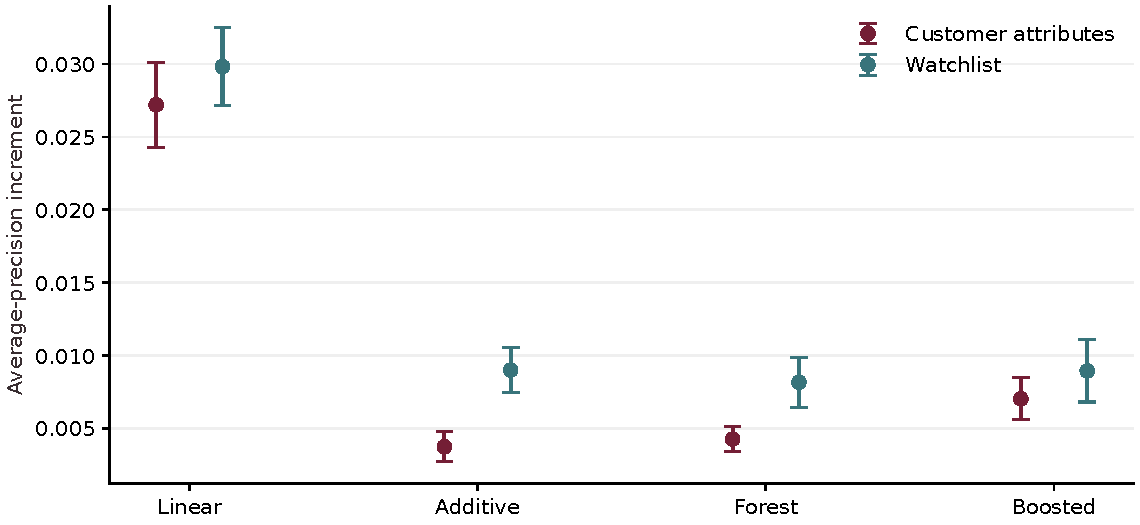
\includegraphics[width=.94\linewidth]{figures/ladder.pdf}\caption{AP increments from attributes and the watchlist across the four models. Intervals are computed on paired within-world increments. The four labels denote model families, not a validated scalar scale of capacity.}\end{figure}

\subsection{Auxiliary signal remains useful in unfavorable regimes}
The full surface appears in Table~\ref{tab:surface}. When the auxiliary block is made uninformative, the AP gains are near zero or slightly negative. Negative realized gains are possible because fitting additional noise variables changes a finite-sample estimator; information nesting does not guarantee monotonically increasing fitted performance. When auxiliary signal is high, all four models benefit across every tested behavioral regime. Under low behavioral recoverability and high auxiliary signal, the full-access AP gains are about 0.138 for logistic regression and 0.038 for unconstrained boosting. The latter is materially larger than its default gain of 0.016 in the native AP units.
\begin{table}[htbp]\centering\scriptsize
\caption{Full-access AP increment across the executed 5\% prevalence surface. Low/high behavior means low/high recoverability. Default mid/mid has 20 worlds; other cells have 10. Brackets are pointwise 90\% intervals.}\label{tab:surface}
\begin{tabular}{llcccc}\toprule Behavior & Auxiliary & Linear & Additive & Forest & Boosted \\\midrule
Low & Low & -0.002 [-0.003, -0.002] & -0.000 [-0.000, 0.000] & -0.000 [-0.001, 0.001] & 0.001 [-0.000, 0.002] \\
Low & Mid & 0.059 [0.054, 0.064] & 0.012 [0.009, 0.015] & 0.013 [0.010, 0.016] & 0.015 [0.012, 0.019] \\
Low & High & 0.138 [0.128, 0.148] & 0.045 [0.039, 0.050] & 0.036 [0.031, 0.041] & 0.038 [0.034, 0.042] \\
Mid & Low & -0.003 [-0.003, -0.002] & -0.000 [-0.000, 0.000] & -0.001 [-0.002, -0.000] & -0.001 [-0.002, 0.000] \\
Mid & Mid & 0.057 [0.053, 0.061] & 0.013 [0.011, 0.015] & 0.012 [0.010, 0.014] & 0.016 [0.014, 0.018] \\
Mid & High & 0.123 [0.112, 0.135] & 0.040 [0.033, 0.047] & 0.034 [0.028, 0.039] & 0.035 [0.029, 0.040] \\
High & Low & -0.002 [-0.003, -0.002] & -0.000 [-0.000, 0.000] & -0.001 [-0.001, 0.000] & -0.000 [-0.001, 0.001] \\
High & Mid & 0.049 [0.044, 0.053] & 0.007 [0.004, 0.010] & 0.007 [0.005, 0.010] & 0.007 [0.005, 0.009] \\
High & High & 0.116 [0.107, 0.125] & 0.032 [0.029, 0.035] & 0.027 [0.022, 0.031] & 0.026 [0.021, 0.030] \\
\bottomrule
\end{tabular}
\end{table}
\begin{figure}[htbp]\centering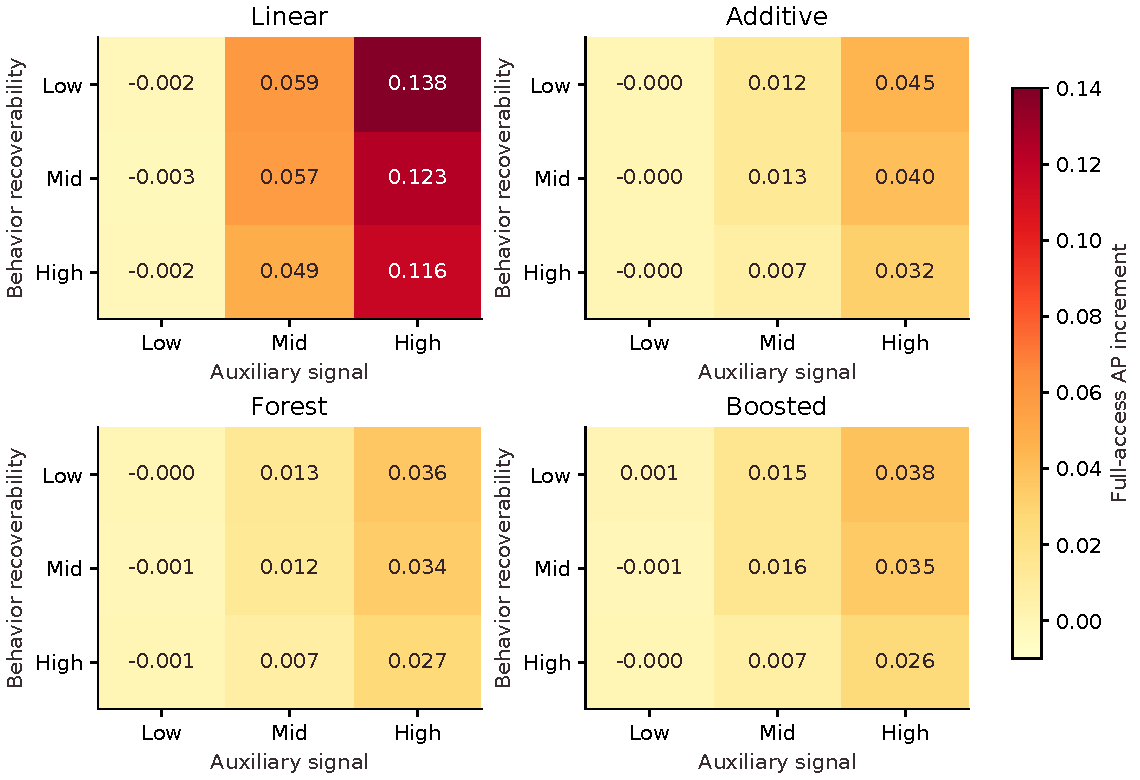
\includegraphics[width=\linewidth]{figures/surface.pdf}\caption{The combined AP increment above linkage by generated regime. The common color scale preserves the relative magnitude across models. Every panel is at the executed 5\% prevalence; it is not the 3\% surface named in the original plan.}\end{figure}

The surveillance-favoring positive control increases the AP gain for every model (Appendix~\ref{app:controls}). It demonstrates that the harness can return an unfavorable region for the proposed privacy separation. With only two worlds, its interval is imprecise and the control does not map a population effect. It also contradicts any blanket assertion that a capable detector eliminates the value of auxiliary information.

Changing prevalence alters the comparison again (Appendix~\ref{app:prevalence}). A fixed 5\% review budget exceeds the nominal illicit prevalence in the 1\% and 3\% settings, and the relationship between recall, precision, AP, and additional misses changes accordingly. The results therefore cannot be scaled from one prevalence to another by multiplying a headline detection percentage.

\subsection{Budget saturation and diagnostic results}
The excluded pilot's resolution scan is reported in Table~\ref{tab:resolution}. At budgets of 50, 100, and 200, the boosted T2--T4 contrast is exactly zero in all pilot replicates. At 500 it is nonzero in aggregate and no replicate is marked saturated by the pilot diagnostic. The scan explains the operating-point choice and prevents the zero at a small budget from being read as strong privacy evidence.
\begin{table}[htbp]\centering\small
\caption{Excluded 20-world pilot, not independent-population results. Positive differences are extra misses without the full auxiliary block. ``Saturated'' denotes both boosted tiers selecting only positive cases at that budget.}\label{tab:resolution}
\begin{tabular}{rccc}\toprule Reviews/10,000 & Boosted difference & Logistic difference & Boosted saturated \\\midrule
50 & 0.00 & 0.00 & 100\% \\
100 & 0.00 & 0.05 & 100\% \\
200 & 0.00 & 1.10 & 100\% \\
300 & 0.00 & 7.20 & 90\% \\
400 & 0.55 & 25.35 & 65\% \\
500 & 7.75 & 31.65 & 0\% \\
625 & 11.65 & 31.25 & 0\% \\
1000 & 8.40 & 19.50 & 0\% \\
\bottomrule
\end{tabular}
\end{table}

The retrospective permutation controls and deterministic reproductions are reported in Appendix~\ref{app:controls}. Permutation results test a specific implementation failure: predictive ranking should disappear when the entity labels are shuffled consistently throughout the learning pipeline. They cannot establish that the original synthetic populations resemble a field deployment. The deterministic checks likewise establish that the archived outcomes are generated by the supplied code and pins; they do not turn an illustrative DGP into external validation.

\section{Discussion}
\subsection{The scientific contribution and its limits}
The evidence answers a restricted but operationally interpretable question. In these synthetic populations, at these budgets, how much does a fixed learner gain from customer attributes and watchlist membership after wallet linkage is supplied? The answer differs substantially between logistic regression and nonlinear models, and changes across signal regimes. Decomposing the result prevents three common conflations: linkage with naming, customer attributes with watchlists, and good average ranking with low missed-case cost at the review budget.

The smaller nonlinear increment is consistent with behavioral features acting as substitutes for some auxiliary predictors. It is not proof that a model infers civil identity, reconstructs all relevant customer information, or makes data collection unnecessary. Several mechanisms remain compatible with the pattern: better estimation of marginal nonlinear effects, regularization, model-specific interactions, and remaining AP headroom. The additive comparison narrows the interpretation beyond a two-model comparison, but does not distinguish these mechanisms fully.

Neither the synthetic label prevalence nor the class-conditional auxiliary distributions have been calibrated to a particular payment institution. The design uses a single generator family, with several parameterized regimes rather than independent models of illicit behavior. It contains no adaptive laundering response to deployment, cross-jurisdiction transfer of a trained detector, investigator feedback, or measurement of discriminatory outcomes. Model fitting assumes the supplied historical labels are available and correct. The confidence intervals quantify simulation variation under these assumptions; they do not quantify uncertainty about the assumptions themselves.

The oracle linkage assumption is particularly consequential. False merges and false splits would change the feature matrix, training labels, ranking units, and alert costs. An erroneous merge can even make optimistic entity-coverage metrics look better by crediting several entities to one alert. T2-oracle is therefore an idealized reference, not a proven numerical upper bound on every metric under arbitrary linkage errors. We do not claim a resolved-linkage sensitivity analysis has been performed. A field study should score noisy clusters using both an entity-coverage rule and a conservative rule that credits at most one positive per reviewed cluster, with explicit handling of split fragments.

\subsection{Separating wallet linkage from civil-identity resolution}
The measurement motivates an institutional design question rather than licensing one architecture. Let $w\mapsto c$ associate wallets with a monitoring cluster, and let $c\mapsto id$ associate that cluster with civil identity. A routine monitoring service may need the first map and behavioral features without receiving the second. The experiment supplies $w\mapsto c$ perfectly and measures selected auxiliary fields; it does not implement either access-control path.

Our candidate design uses a payment service provider to conduct onboarding checks and retain the customer dossier. It issues a credential binding approved wallet keys to a cluster identifier and an epoch. A holder presents a proof of credential possession for an authorized monitoring context, revealing the cluster required for scoring while withholding civil attributes. Anonymous-credential signature protocols provide relevant building blocks \citep{CL}; this paragraph specifies intended information flow, not an implemented credential protocol or a proof of compositional security.

Civil resolution follows a separate case process: a requesting authority records a case and legal basis, and a specified threshold of independent opening authorities authorizes the escrowed resolution. The request, authorization, and opening are logged for independent audit. Epoch changes require an explicit policy for retention and cross-epoch linkage; issuing multiple unlinked credentials must be governed through onboarding controls. Neither the threshold nor the epoch length is selected by the detection experiment.

These intended controls have limited reach. The issuer retains the dossier and can potentially relink offline; colluding opening authorities can meet the threshold; validators can leak routing metadata; and stable clusters permit extensive behavioral tracking without names. Consequently, we claim neither anonymity nor unlinkability, and no universal prohibition on unilateral access by an issuer. The design seeks to restrict the routine scoring service's access and create accountable resolution. Court-compelled disclosure and institution-specific obligations remain possible. The earlier claim that the architecture prevents bulk surveillance is also too strong: cluster-level surveillance is explicitly retained.

\subsection{What a distributed ledger would add}
A fair baseline is a centralized payment system with separate credential, monitoring, and resolution roles, cryptographic controls, and independently witnessed audit logs. A distributed ledger without information separation does not create the separation merely by distributing storage. A permissioned ledger with separate resolution could provide multiparty custody of settlement and opening records, conditional on its consensus and corruption assumptions. It would also introduce replication, governance, and availability costs. We have not measured those costs or verified a ledger protocol.

The relevant distinction is thus which organizations can authorize access or alter evidence, not whether a database is called a blockchain. A centralized system can also use independent witnesses and threshold keys. The experiment selects neither alternative. The distributed version is worth considering only where joint institutional custody and resistance to unilateral log alteration are required and the corresponding trust assumptions are credible. This restricted comparison keeps the empirical contribution applicable beyond a particular ledger implementation.

\subsection{Compliance functions remain assigned to institutions}
FATF Recommendations 10, 11, 16, 20, and 21 respectively address customer due diligence, records, payment transparency, suspicious-transaction reporting, and tipping-off/confidentiality \citep{FATF}. In the candidate allocation, providers retain identity and transaction records, exchange required payment information through authorized channels, and remain responsible for reporting; the monitoring service supplies scores. Separating routine scoring from identity access creates no exemption from those duties. The applicable national rules and information flows would still need to be mapped for a deployment. The earlier notification-and-abandonment mechanism is excluded from this candidate because revealing investigation status can conflict with confidentiality and create a probing channel. We make no claim that the design complies with a jurisdiction's law or that a detection estimate determines the lawful scope of identification.

\subsection{Illustrative PET--AML workload simulation}
An earlier manuscript component modeled a payment-service stack with assumed communication volumes, service times, queues, limits, and escalation rules. It is distinct from the detection experiments. Re-running both amount-generation configurations exposes substantial sensitivity (Appendix~\ref{app:pet}). The original configuration rejects 14,713 of 40,000 transfers and creates 27 case packets. Tier-aware amounts reject 3,375 and create 592 packets. The estimated aggregate MPC workload rises from 0.38 to 0.55 hours. Presenting the smaller rejection rate together with the original 27-packet count mixes incompatible configurations.

We retain the complete comparison as an illustrative engineering appendix because it documents the existing simulator and its correction. These are outputs from a two-day, single-seed queue model, not measurements of deployed zero-knowledge proofs, MPC, throughput, or AML effectiveness. They provide no independent empirical support for the article's detection result and no evidence that the institutional design has been implemented.

\section{Conclusion}
In the specified synthetic payment populations, customer attributes and watchlist membership improve detection above oracle pseudonymous linkage for both fixed model families. Their combined operational value is substantially smaller for gradient boosting than for logistic regression, while the four-model experiment shows that additive nonlinear models already display much of that pattern. Stronger auxiliary signals benefit every model. These findings support measuring information increments at a stated review budget, with explicit representation and learner choices, before drawing conclusions about data collection. They do not establish a general privacy--detection equivalence, a threshold for acceptable missed cases, or a validated CBDC architecture.

\section*{Declarations}
\paragraph{Author contributions.} Murad Farzulla: conceptualization, methodology, detection-pipeline development, analysis, and manuscript preparation. Andrew Maksakov: PET--AML stack design, simulator development, and original writing of that component. These descriptions preserve the existing substantive contribution; this draft does not certify final co-author endorsement.
\paragraph{Funding and interests.} The existing manuscript records no external funding and no competing interests. These declarations are carried forward for review.
\paragraph{Data and code.} All empirical populations in this article are synthetic. The August baseline code and archived results are identified by commit \texttt{304a3fe} in \url{https://github.com/andrewmaksakov/CBDC}. The September correction, complete reproduction instructions, raw diagnostic outputs, generated tables, and manuscript sources are supplied in the accompanying review archive. The revised archive is a local candidate at the time of drafting; a public September code release is not claimed. The intended maintained repository is \url{https://github.com/dissensus-ai/CBDC}; its public contents must be synchronized before publication of this revision.
\paragraph{AI assistance.} Claude (Anthropic) and ChatGPT/Codex (OpenAI) assisted earlier and current analysis, source checking, code review, and manuscript preparation. The September revision includes an automated full reproduction of the independent-population experiment and explicit correction of the gatekeeping error. AI assistance is not independent author endorsement; responsibility for a released manuscript remains with its authors.

\appendix
\section{Model specifications and reproduction}\label{app:models}
The independent-population logistic model uses standardization, balanced class weights, and \texttt{max\_iter=2000}; boosting uses scikit-learn's histogram gradient boosting defaults with balanced class weights. The seed enters model randomness after deterministic conversion into scikit-learn's accepted integer range. The supplied environment and original seed list are required for exact reproduction.

The ladder's logistic grid uses $C=0.01,0.1,1,10$. Features are standardized; the solver is \texttt{lbfgs} with at most 5,000 iterations. Additive and unconstrained histogram boosting each use learning rates $\{0.05,0.10\}$ crossed with maximum leaf counts $\{15,31\}$; the additive model forbids feature interactions. The random forest uses 400 trees with feature subsampling $\{\texttt{sqrt},0.5\}$ crossed with minimum leaf sizes $\{1,5\}$. All families use balanced class weights. AP selects a configuration in three inner folds on T4 for each outer fold, which is reused in T1--T4. These are shared tuning rules, not equal training time or equal effective complexity.

The review archive's \texttt{REPRODUCE.md} gives commands for four tasks: re-aggregate immutable August records; reproduce all 52 independently generated train/test pairs; reproduce the selected full-ladder unit and the retrospective permutation controls; and build the manuscript from its minimal source archive. Original records remain intact. SHA-256 checksums identify their inputs and the submitted candidate artifacts. Public-data loaders are not represented as completed external validation.

\section{Control and reproduction outputs}\label{app:controls}
\begin{table}[H]\centering\small
\caption{Auxiliary-favoring positive control: full-access AP increment, two independent worlds per model, pointwise 90\% intervals. Small sample size limits precision.}
\begin{tabular}{lc}\toprule Model & $\Delta_F(\AP)$ \\\midrule
Linear & 0.422 [0.403, 0.440] \\
Additive & 0.134 [0.085, 0.184] \\
Forest & 0.129 [0.089, 0.168] \\
Boosted & 0.117 [0.096, 0.137] \\
\bottomrule
\end{tabular}
\end{table}
\begin{table}[H]\centering\small
\caption{Retrospective label-permutation diagnostics: T4 AUC across 22 worlds spanning the tested regimes. The range describes observed world variation, not a confidence interval.}
\begin{tabular}{lcc}\toprule Model & Mean AUC & Observed range \\\midrule
Linear & 0.492 & 0.455--0.525 \\
Additive & 0.502 & 0.449--0.538 \\
Forest & 0.493 & 0.432--0.520 \\
Boosted & 0.494 & 0.462--0.534 \\
\bottomrule
\end{tabular}
\end{table}
All 22 retrospective permutation worlds completed without failures. Mean T4 AUCs are close to 0.5, with the observed ranges shown above; no formal equivalence-to-chance test was specified. The reproduction evidence records exact equality of all 52 original independent-population raw records, with the H2 interpretation changed to descriptive. The selected ladder replay compares the entire model-output structure, including selected hyperparameters. The negative controls were generated after inspecting the original results and are labeled accordingly. Their small per-regime replication count is adequate for a basic leakage check but does not establish equivalence to a theoretical chance-performance distribution.

\section{Prevalence sensitivity}\label{app:prevalence}
\begin{table}[H]\centering\scriptsize
\caption{Default behavioral and auxiliary regimes at three prevalences. Full-access AP increments with pointwise 90\% intervals. The 1\% and 3\% cells have 10 worlds each; the 5\% cell reuses the 20-world default result.}
\begin{tabular}{lcccc}\toprule Prevalence & Linear & Additive & Forest & Boosted \\\midrule
1\% & 0.090 [0.069, 0.111] & 0.012 [0.006, 0.019] & 0.008 [0.004, 0.012] & 0.009 [0.004, 0.015] \\
3\% & 0.067 [0.060, 0.075] & 0.013 [0.011, 0.015] & 0.012 [0.009, 0.014] & 0.019 [0.015, 0.022] \\
5\% & 0.057 [0.053, 0.061] & 0.013 [0.011, 0.015] & 0.012 [0.010, 0.014] & 0.016 [0.014, 0.018] \\
\bottomrule
\end{tabular}
\end{table}

\section{Complete simulator configuration comparison}\label{app:pet}
Both columns use 40,000 simulated transfers over two days with seed 7. Only the tier-aware amount-generation option changes. Counts, latency summaries, and modeled resource totals are reported together to avoid combining rows from different configurations.
\begin{table}[H]\centering\small
\caption{PET--AML simulator outputs. All times and resource totals are modeled quantities; no cryptographic deployment benchmark was run.}
\begin{tabular}{lrr}\toprule Quantity & Original amounts & Tier-aware amounts \\\midrule
Transfers generated & 40,000 & 40,000 \\
Settled & 25,287 & 36,625 \\
Rejected & 14,713 & 3,375 \\
Sanctions blocks (included in rejections) & 82 & 82 \\
Tier-limit rejections & 14,631 & 3,293 \\
Escalation case packets & 27 & 592 \\
Modeled PSI communication (MB) & 156,851.87 & 156,851.87 \\
Modeled proof bytes & 20,438,016 & 20,438,016 \\
Modeled aggregate MPC hours & 0.38 & 0.55 \\
Mean settled latency (ms) & 536.78 & 536.57 \\
Median settled latency (ms) & 510.54 & 510.28 \\
90th percentile settled latency (ms) & 768.08 & 765.59 \\
99th percentile settled latency (ms) & 1,137.31 & 1,136.14 \\\bottomrule\end{tabular}
\end{table}
The archived logs additionally report queue waits and final risk-tier distributions. The number of cases in each column is a consequence of the chosen simulator rules and amount process; the difference does not estimate a treatment effect in an observed payment system.

\bibliographystyle{plainnat}
\bibliography{references}
\end{document}
